\chapter{Génomique des procaryotes : organisation, évolution et fonctions}

Les génomes procaryotes sont souvent décrits comme plus simples et plus faciles à étudier que les génomes eucaryotes. La simplicité apparente de ces génomes cache en réalité des mécanismes complexes. Dans cette partie, je décrirai les mécanismes les plus connus et les plus répandus.

\section{Structure et organisation des génomes procaryotes}
\label{sec:structure_org}

%Le génome correspond à l'ensemble du matériel génétique, c.-à-d., des éléments qui seront hérités par les cellules de la génération suivante. Le génome, c'est aussi la structure de base qui va contenir l'ensemble des informations nécessaires au fonctionnement et à la survie de la cellule. Ces informations sont contenues dans la molécule d'ADN, ce qui nous amène à la structure primaire du génome, la séquence nucléotidique. Cette séquence est souvent circulaire chez les procaryotes et est de petite taille, quelques centaines de milliers de bases, mais certains génomes peuvent atteindre plusieurs millions de bases\footnote{En bioinformatique, on utilise l'unité base (b) ou paire de base (pb), pour mesurer la taille d'un génome. Un génome procaryote sera donc compris entre 100 kb et 10 Mb. Pour comparaison, le génome humain mesure environs 3 Gb.} (\autoref{fig:genome_size}).

Le génome procaryote correspond à la séquence de nucléotides qui composent la molécule d'ADN qui est bicaténaire, \textit{i.e.}, composée de deux brins antiparallèles reliés par complémentarité des bases (A$\leftrightarrow$T, C$\leftrightarrow$G). Le génome est souvent circulaire et de petite taille, quelques centaines de milliers de bases, mais certains génomes peuvent atteindre plusieurs millions de bases\footnote{En bioinformatique, on utilise l'unité base (b) ou paire de base (pb), pour mesurer la taille d'un génome. Un génome procaryote sera donc compris entre 100 kb et 15 Mb. Pour comparaison, le génome humain mesure environs 3 Gb.} (\autoref{fig:genome_size}). Enfin, le génome se divise en deux grandes catégories : l'ADN codant et l'ADN non codant.

\begin{figure}[htbp]
    \centering
    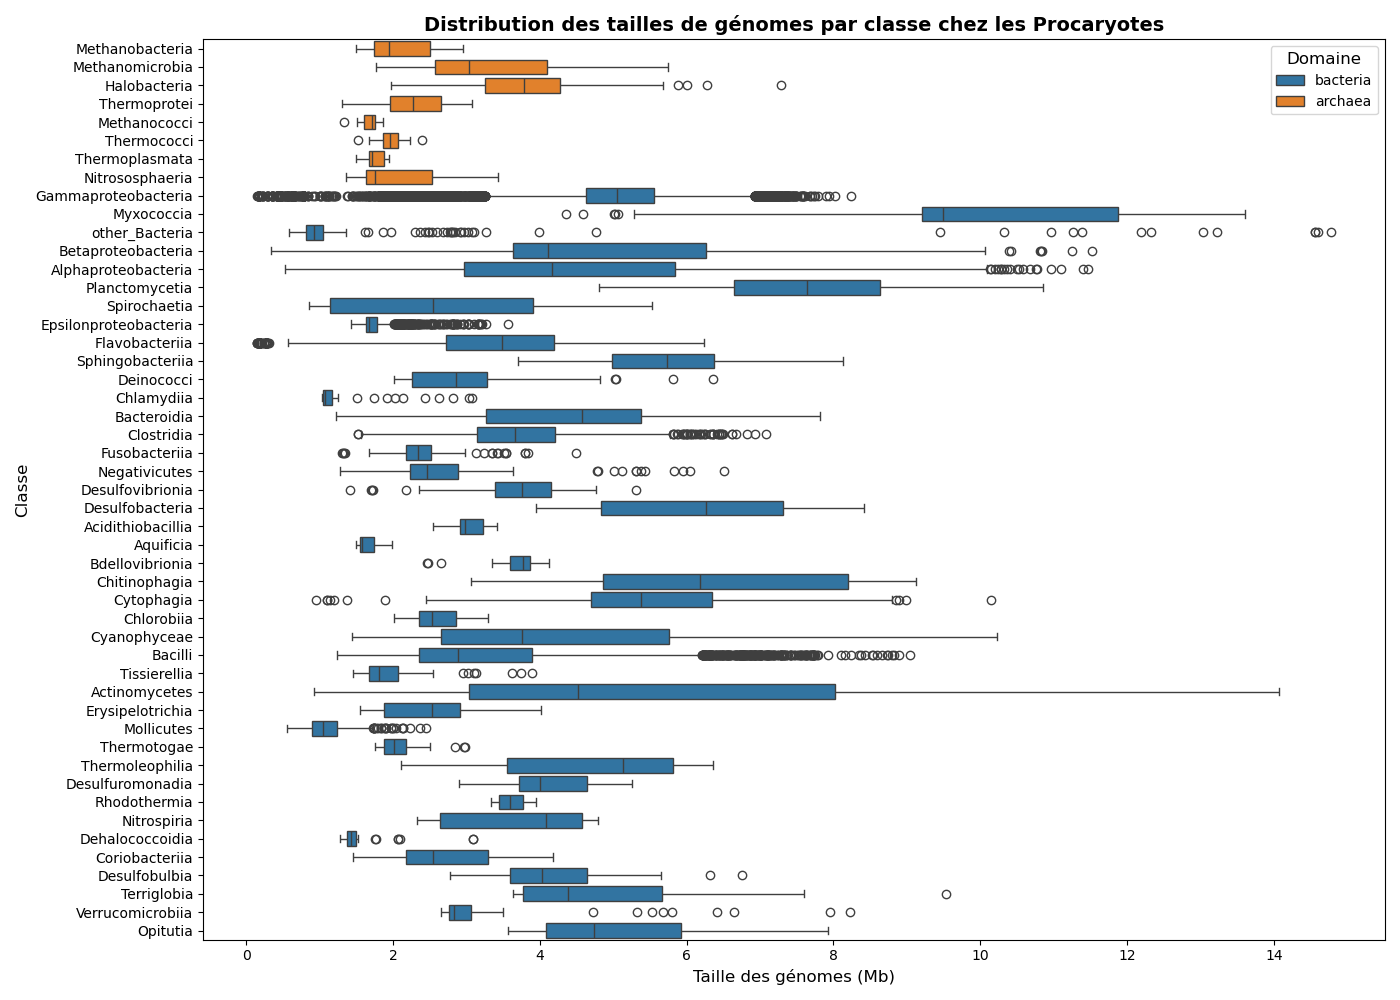
\includegraphics[width=\textwidth]{images/genome_sizes_boxplot.png}
    \caption[Distribution de la taille des génomes chez les procaryotes]{Distribution de la taille des génomes (en base) par classe chez les procaryotes. Les données utilisées proviennent de RefSeq version 28 janvier 2025.}
    \label{fig:genome_size}
\end{figure}

\newpage
\subsection{Constituant du génome : le codant et le non codant}
\label{sec:gene}
%\subsection{Organisation génique des procaryotes}
Chez les procaryotes, le génome est majoritairement constitué de séquences codantes (entre 85 et 90 \%), ce qui compense leur petite taille. 
L'ADN codant correspond à des blocs de nucléotides d’environ 1 kb. Ces blocs codants sont appelés gènes et ils jouent un rôle essentiel puisqu’ils contiennent l’information nécessaire à la production des protéines impliquées dans toutes les réactions cellulaires (cf. \autoref{sec:fn_reg}). De plus, l’ADN procaryote étant bicaténaire, chaque gène peut alors être lu dans les deux directions (sur le brin direct ou complémentaire), doublant ainsi la quantité d'information sur une position précise du génome (locus). 

Dans le génome, les gènes ne sont pas répartis aléatoirement. Ceux qui codent une fonction biologique similaire sont souvent regroupés dans un  contexte génomique. La conservation de l'ordre des gènes, appelé aussi synténie, peut varier entre les génomes, mais les gènes restent dans le même contexte \cite{lathe_gene_2000}, on parle alors de contexte conservé ou de synténie conservée. De plus, la position des gènes par rapport à l'origine de réplication (Ori: région où commence la réplication de l'ADN) à aussi son importance. Il a été montré que chez les bactéries avec un fort taux de division, les gènes ayant un rôle essentiel sont plus proches de l'Ori afin d'être plus fortement exprimés \cite{sharp_chromosomal_1989,vieira-silva_systemic_2010}.
%Les gènes sont soumis à des mécanismes de régulation communs (cf. \autoref{sec:fn_reg}).

Pour finir, les gènes peuvent être classés selon l’importance de leur fonction pour la survie de la cellule. Les gènes indispensables au cycle de vie d'une cellule, par exemple la réplication de l’ADN, la transcription, ou la traduction, sont dits "essentiel" et se distinguent des gènes "accessoires", qui codent pour des fonctions d'adaptation à des conditions particulières, comme la résistance aux antibiotiques, la défense contre les virus ou des transformations métaboliques spécifiques.



%Le génome est divisé en sous-unité que l'on appelle gène. Le gène contient l'information nécessaire pour produire une protéine qui réalisera une fonction dans la cellule (\autoref{fig:gene2prod}), on dit que le gène code pour une protéine. Pour ça, l'ADN est d'abord transcrit en une molécule d'ARNm, qui sera traduite en protéine (gène A sur la \autoref{fig:genome_size}) par des complexes protéine/ARN, les ribosomes. Ces protéines correspondent à une chaîne d'acides aminés, que l'on peut représenter sous forme de séquence. Pour passer d'un gène à une protéine, on utilise une table de correspondance que l'on appelle code génétique où 3 nucléotides correspondent à 1 acide aminé. En moyenne, une protéine contient 300 acides aminés, ramenant la taille des gènes à environ 1 kb. Enfin, comme indiqué sur la partie haute de la \autoref{fig:genome_size}, les génomes procaryotes sont majoritairement codants, ce qui veut dire que presque tout l'ADN peut être divisé en gènes, et donc qu'il y a environ entre 100 et 10 000 gènes dans les génomes en fonction de leur taille. En mettant toutes ces informations en perspective, on comprend que la petite taille des génomes procaryotes est compensée par son fort taux de gènes, et qu'ainsi, il contient l'ensemble des protéines nécessaires à la survie de la cellule. 


\begin{figure}[htbp]
    \centering
    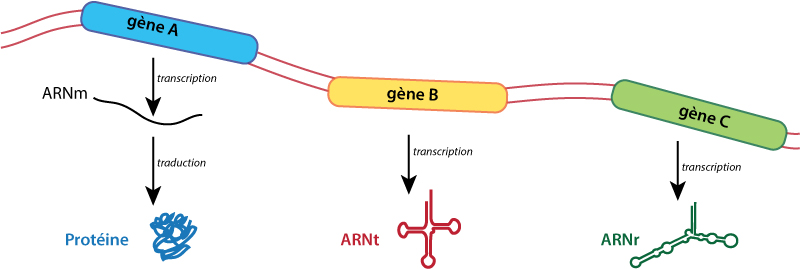
\includegraphics[width=\linewidth]{images/gene2prot.jpg}
    \caption[Produit d'un gène]{Produit d'un gène dans la cellule. Un gène est d'abord transcrit en ARN. Si l'ARN transcrit est dit messager (ARNm), il sera ensuite traduit en protéine, sinon l'ARN produit (ARNt, ARNr, miARN, ....) aura un rôle spécifique dans des processus cellulaire. Copié de RNBio, Sorbonne université. \url{https://rnbio.sorbonne-universite.fr/genetique_genotype1}}
    \label{fig:gene2prod}
\end{figure}

L'ADN non codant constitue une part tout de même importante du génome et selon l'adage "la nature a horreur du vide"\footnote{Citation d'Aristote qui, répondant à Démocrite, dit que l'univers ne pouvait être rempli de vide. On sait aujourd'hui que Démocrite avait raison, mais dans le cas des génomes procaryote, l'idée fonctionne.}. Cet ADN non codant, n'est donc pas inutile et renferme également des fonctions essentielles à la vie de la cellule.
Tout d'abord, on retrouve les séquences d'ADN qui seront transcrits en ARN ribosomiques (ARNr) ou ARN de transfert (ARNt). Ces ARN sont indispensables pour la construction de la chaîne d'acide aminée de la protéine. Ces séquences d'ADN sont considérée aussi comme des gènes et selon les sources comme faisant partie du codant. Cependant, d'un point de vue sémantique et biologique ces gènes ne code pas, les nucléotides sont copiés d'une forme d'acide désoxyribonucléique en une forme d'acide ribonucléique. L'ADN non codant renferme d'autres formes d'ARN, comme les microARN et les ARN interférents (miARN et siARN). Ces ARN sont aujourd'hui considérés comme des acteurs clés dans la régulation des fonctions biologiques \cite{backofen_bioinformatics_2014,watkins_regulatory_2019}, mais aussi dans d'autres processus comme le système immunitaire \cite{bobadilla_ugarte_argonaute_2023}.

L'ADN non codant n'a pas uniquement le rôle de contenir les séquences transcrites en ARN, il contient aussi d'autres éléments régulateurs de l'expression des gènes contenus dans l'espace intergénique (cf. \autoref{sec:fn_reg}). On retrouve aussi dans l'ADN non codant des séquences répétées, comme les séquences d'insertion (IS) qui se déplace dans le génome, ou les séquence CRISPR (Régions composées de répétitions palindromiques et d’espacers, impliquées dans le système immunitaire adaptatif des bactéries) \cite{jansen_identification_2002,bolotin_clustered_2005}. Il existe tout de même une partie d'ADN non codant qui n'a aucun rôle, ces séquences sont des vestiges d'anciens gènes qui au cours de l'évolution ont perdu leur fonction (cf. \autoref{sec:dyn_evo}). Pour terminer, c'est aussi dans le non-codant que l'on va retrouver des éléments essentiels dans la réplication et l'évolution des génomes procaryotes : l'origine de réplication (Ori) et les éléments génétique mobile (MGE). 
%Tous les gènes ne sont pas traduits en protéine, une partie de ces gènes seront transcrit dans des formes d'ARN ayant un rôle dans la régulation et le fonctionnement de la cellule. Les ARN ribosomiques (ARNr), sont les constituants fondamentaux de la structure et du fonctionnement des ribosomes. Ils vont interagir avec les ARN de transfert (ARNt), qui acheminent les acides aminés vers les ribosomes pour traduire l'ARNm en protéine. D'autres ARN, comme les microARN et les ARN interférents (miARN et siARN), interviennent dans la régulation de l'expression des gènes. Cette liste non exhaustive montre la diversité des ARN et beaucoup étaient encore considérés il y a peu comme des produits secondaires sans réelle fonction. Aujourd'hui, ils sont considérés comme des acteurs clés dans la régulation des fonctions biologiques \cite{watkins_regulatory_2019,backofen_bioinformatics_2014}, mais aussi dans d'autres processus comme le système immunitaire \cite{bobadilla_ugarte_argonaute_2023}

\subsection{Réplicons et mécanismes de réplication dans les génomes procaryotes}
\label{sec:replicons}
La multiplication des cellules procaryotes s'effectue par division, où une cellule mère donne naissance à deux cellules filles. Afin de transmettre l’information génétique aux cellules nouvellement formées, l’ADN doit être répliqué, \textit{i.e.}, copié de manière exacte. Le terme réplicon désigne l’ensemble des molécules d’ADN capables de se répliquer de façon autonome. Un réplicon contient ainsi tous les éléments nécessaires à l’exécution et à la régulation de la réplication. Chaque réplicon contient une séquence d’ADN spécifique, appelée origine de réplication (Ori), où commence le processus de réplication.

La forme principale de réplicon dans la cellule procaryote est le chromosome. Le chromosome, souvent circulaire et replié, constitue le plus grand réplicon en termes de paires de bases. Chez les procaryotes, le chromosome est généralement unique, bien que d'autres réplicons puissent coexister au sein de la cellule.

Une seconde forme de réplicon, connue pour son rôle dans l’évolution (voir \autoref{sec:evo_hz}), est le plasmide \cite{lederberg_gene_1946,lederberg_sex_1953}. Les plasmides, souvent circulaires et de taille inférieure à celle du chromosome, sont indépendants de ce dernier. En tant que réplicons, ils se répliquent de manière autonome et peuvent être présents en grand nombre dans une cellule. L’origine de réplication des plasmides diffère de celle des chromosomes. Par ailleurs, les plasmides peuvent accumuler de nouvelles séquences et augmenter en taille, prenant alors la forme de mégaplasmides (\autoref{fig:replicon}).

Chez la majorité des procaryotes, le chromosome contient les gènes essentiels, tandis que les plasmides portent des gènes accessoires. Cependant, certaines formes de réplicons oscillent entre chromosome et plasmide. Par exemple, chez \textit{Rhodobacter sphaeroides}\footnote{Bactérie présente dans les lacs profonds et les eaux stagnants. Elle est capable de réaliser la photosynthèse et son métaolisme est très diversifié et donc très utilisé en biotechnologie} et \textit{Vibrio cholerae}\footnote{Bactérie responsable du choléra, on la retrouve dans l'eau et peut se propager entre humain en utilisant la transpiration}, un second chromosome a été identifié \cite{suwanto_physical_1989,trucksis_vibrio_1998}. Aujourd'hui, ces chromosomes secondaires sont distingués d'une forme de réplicons proche, le chromide \cite{harrison_introducing_2010}. Les chromides, de taille intermédiaire entre un plasmide et un chromosome principal, contiennent des gènes essentiels à la cellule. Ces gènes présentent une proximité phylogénétique avec les espèces du même genre, contrairement à ceux du chromosome principal, qui sont conservés au-delà du genre. En revanche, en termes de mécanismes de réplication et de séquences Ori, les chromids utilisent des systèmes de type plasmidique.

L’usage des termes chromosome secondaire, chromid et mégaplasmide demeure actuellement peu standardisé dans la littérature \cite{hall_what_2021}. Plusieurs critères permettent néanmoins de les distinguer. Le premier repose sur le contenu génétique : les mégaplasmides n’abritent pas de gènes essentiels, contrairement aux chromosomes secondaires et aux chromids. Le second critère est la composition en nucléotides, qui est plus proche de celle du chromosome principal pour les chromids et les chromosomes secondaires. Enfin, leur origine évolutive les différencie : le chromosome secondaire résulte de la scission d’un chromosome ancestral en un chromosome principal et un secondaire, tandis que le chromid dérive d’un ancien mégaplasmide ayant perdu sa capacité de mobilité (voir \autoref{sec:evo_hz}) et qui a intégré des gènes essentiels (\autoref{fig:replicon}). Les chromides auraient donc plutôt un rôle de réservoir de gènes d'intérêt et d'adaptation améliorant la \textit{fitness} des organismes. Cette vision vertueuse de l'accumulation de gènes s'oppose directement à la vision plus ancienne des plasmides non mobilisable décrits comme parasitant la cellule \cite{levin_accessory_1993,lili_persistence_2007}.

\begin{figure}[htbp]
    \centering
    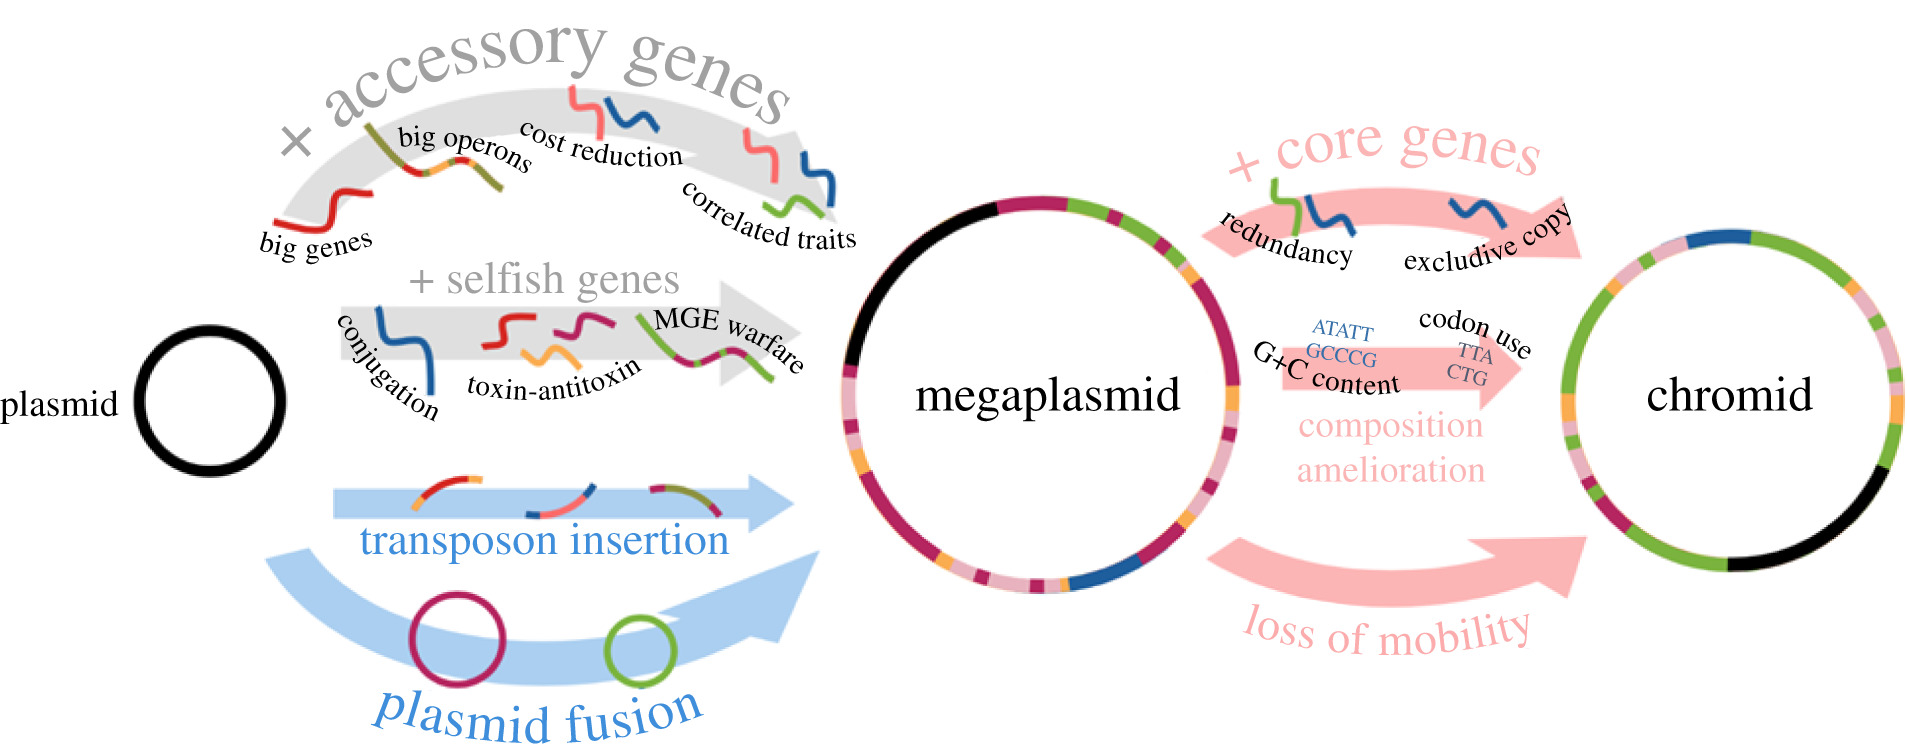
\includegraphics[width=0.8\linewidth]{images/replicon.jpg}
    \caption[Évolution d'un plasmide en chromid]{Schéma simplifié de l'évolution d'un plasmide en megaplasmide et de megaplasmide à chromid. Figure extraite de \cite{hall_what_2021}}
    \label{fig:replicon}
\end{figure}



\newpage
\section{Dynamique évolutive des génomes}
\label{sec:dyn_evo}

La dynamique évolutive des procaryotes est caractérisée par des processus continus de gain, perte et modification de gènes (\autoref{fig:dyna_evo}). La taille des génomes étant restreinte, la perte de gènes peut optimiser le génome en éliminant les séquences redondantes ou non essentielles, favorisant ainsi une efficacité accrue dans des environnements spécifiques. Les modifications génétiques, quant à elles, jouent un rôle crucial dans l'adaptation fine des procaryotes face aux pressions sélectives variées. L'acquisition de nouveaux gènes introduit une diversité génétique, pouvant conférer des traits avantageux, tels que la résistance aux antibiotiques ou la capacité à métaboliser de nouvelles sources de nutriments.

\begin{figure}[htbp]
    \centering
    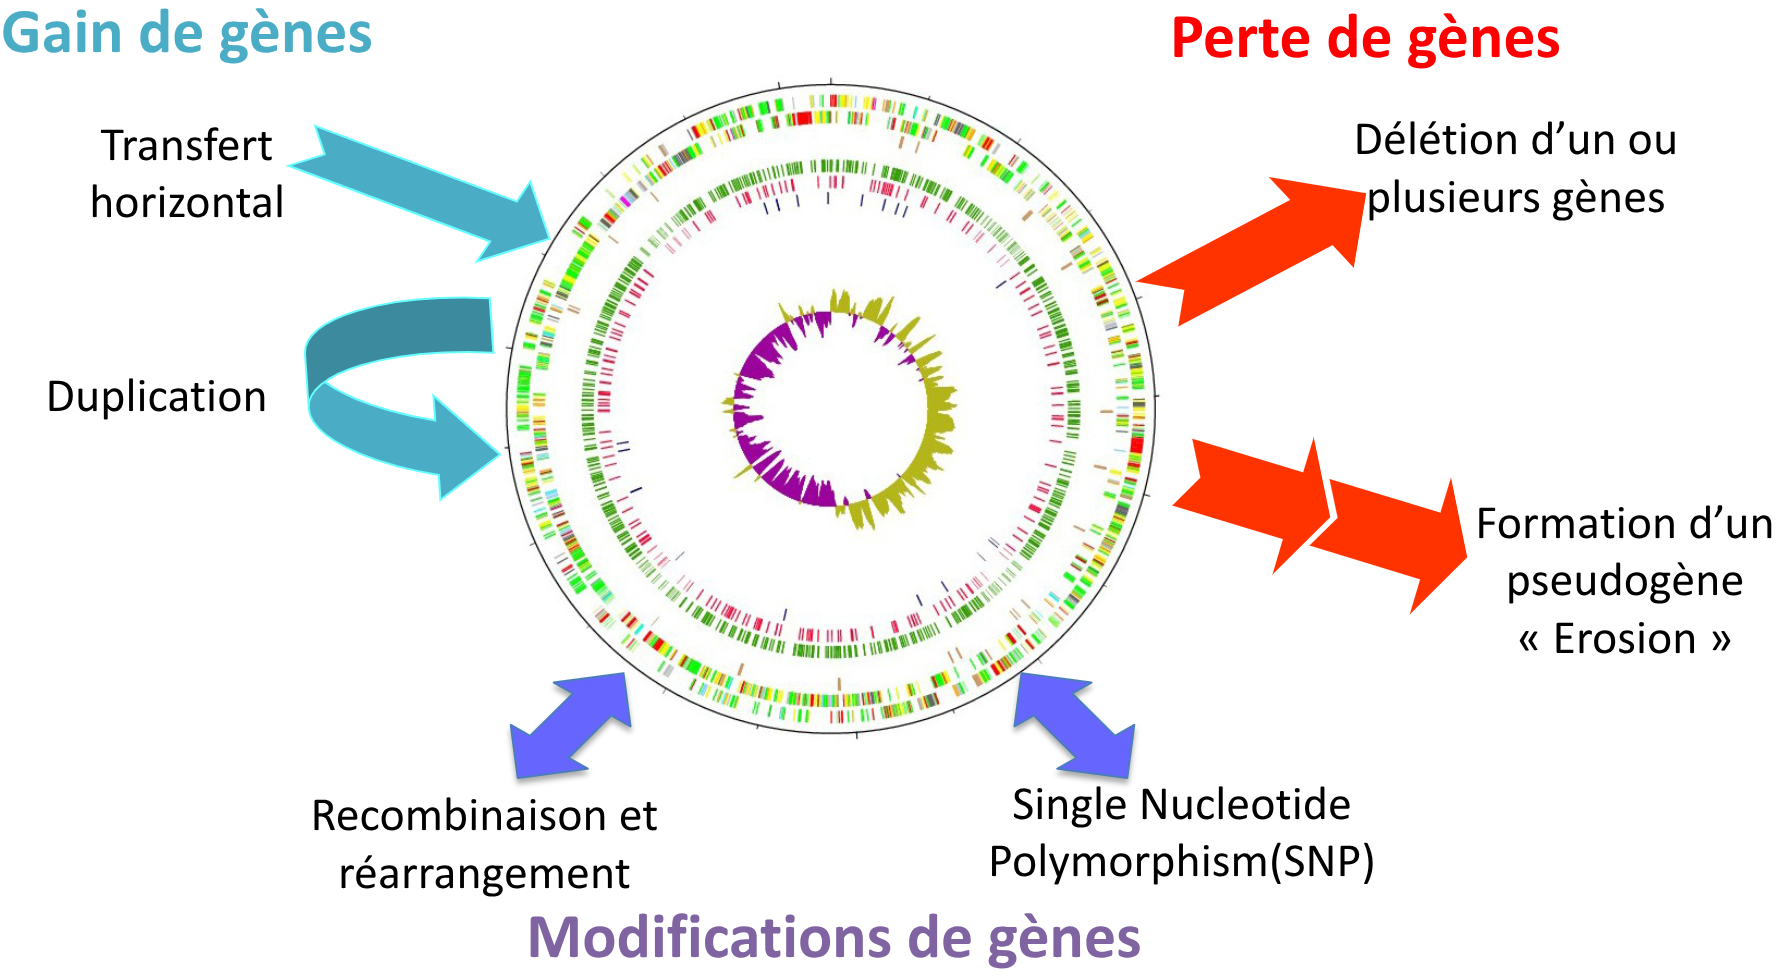
\includegraphics[width=\linewidth]{images/DynamiqueEvo.png}
    \caption[Schéma de la dynamique évolutive des génomes procaryotes]{\textbf{Schéma résumant la dynamique évolutive des génomes procaryotes.} Source LABGeM}
    \label{fig:dyna_evo}
\end{figure}

 Les gènes doivent ensuite être transmis dans la population. Les \textbf{transferts verticaux} permettent de transférer les gènes de génération en génération, assurent la continuité et la stabilité des traits essentiels. Les \textbf{transferts horizontaux} permettent l'échange de gènes entre les organismes, favorisant une diversification rapide des génomes, qui peut radicalement transformer les capacités adaptatives des lignées procaryotes. Cette dynamique complexe façonne la biodiversité procaryote et témoigne de la capacité évolutive exceptionnelle de ces organismes à coloniser une multitude d'écosystèmes.

\subsection{Mécanismes d'évolution par transfert vertical}
\label{sec:evo_ver}
Les mécanismes d'évolution par héritage regroupent les processus menant à une modification du génome entre la cellule mère et la cellule fille. Théoriquement, lors de la division cellulaire, la cellule mère se divise en 2 cellules filles possédant exactement la même information génétique qu'elle. Pourtant, malgré un ensemble de mécanismes de protection et de correction de l'ADN, le génome peut différer entre les cellules mère et fille. Ce sont ces "erreurs" qui vont nous intéresser, car ce sont elles qui sont à l'origine de l'innovation et de la diversité génétique.

\newpage

\subsubsection{Impact des mutations génétiques : SNPs, Indels et pseudogènes}
\paragraph{\textit{Single Nucleotid Polymorphism}}

Un \textit{Single Nucleotide Polymorphism} (SNP) correspond à une modification de la séquence induite par la mutation d'un nucléotide en un autre.
Étant donné que le code génétique est dégénéré\footnote{Un acide aminé peut être codé par plusieurs codons différents.}, la mutation peut ne pas avoir d'impact sur la séquence de la protéine, on dit alors que la mutation est silencieuse ou même sens. Si la modification entraîne un changement d’acide aminé dans la séquence protéique, on parle de mutation faux-sens. Enfin, une mutation est qualifiée de non-sens lorsqu'elle introduit prématurément un codon STOP, interrompant ainsi la traduction et conduisant à une perte de fonction de la protéine. Une telle mutation peut également affecter un site fonctionnel clé (comme un site actif), compromettant l’activité de la protéine. Lorsque l’introduction d’un codon STOP précoce rend un gène non fonctionnel, ce dernier devient un \textbf{pseudogène}, un vestige génomique dépourvu de rôle biologique actif, un phénomène appelé pseudogénisation.

Sur la \autoref{fig:mec_evo}, la première mutation implique un changement de glutamine en histidine, des acides aminés aux propriétés de polarité et de charge différentes. Il s’agit donc d’une mutation faux-sens, qui aura probablement un impact significatif sur la structure de la protéine. En revanche, les deux autres SNPs ne modifient pas l’acide aminé codé, ils sont donc silencieux.

\begin{figure}[htbp]
    \centering
    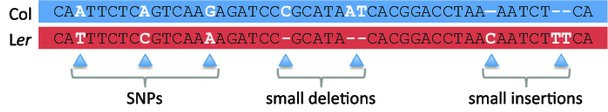
\includegraphics[width=.65\textwidth]{images/Mec_evo.jpg}
    \caption[Identification des SNP et indels entre 2 génomes]{\textbf{SNP et InDels entre deux génomes.} On suppose que le premier codon commence par le premier nucléotide. Figure extraite et adaptée de \cite{qi_detection_2014}}
    \label{fig:mec_evo}
\end{figure}

\paragraph{Indels: insertion, délétion et pseudogènes}

Un indel correspond à l'insertion (In) ou la délétion (del)\footnote{On regroupe l'insertion et la délétion, car sans une analyse phylogénétique, il est impossible de les différencier par comparaison de séquence.} d'un ou plusieurs nucléotides dans la séquence d'un gène. Lorsque la taille de l'indel est un multiple de 3 (insertion ou délétion d'un codon), la séquence protéique peut soit être allongée, soit raccourcie d'un acide aminé, soit coupée de façon précoce si le codon est un codon STOP.

Si la taille de l'indel n'est pas un multiple de 3, il y aura un décalage du cadre de lecture ou \textit{frameshift}. Ce décalage va induire un changement de tous les acides aminés de l'indel à la fin du gène, provoquant avec lui un changement dans la fonction de la protéine ou une inactivation de la fonction. La partie du gène qui n'est pas décalée est alors considérée comme un fragment du gène initial, il est alors qualifié de pseudogène. À nouveau, cette mutation peut être délétère pour la cellule. Sur la \autoref{fig:mec_evo}, les indels sont de taille 1 et 2, elles ne provoquent pas l'apparition d'un codon STOP précoce, mais l'ensemble des acides aminés est modifié.

Les indels vont donc transformer la séquence protéique traduite, pouvant nuire à la fonction de cette dernière et être délétère pour l'organisme. Pour éviter les problèmes liés aux \textit{frameshifts}, il a été montré qu'il existe un fort taux de codon STOP hors du cadre de lecture \cite{tse_natural_2010}. Cette adaptation permettrait de limiter la traduction des protéines mutantes et d'ainsi limiter le coût énergétique pour la cellule. Il a aussi été montré que les \textit{frameshifts} pourraient être à l'origine d'un réservoir d'adaptation à l'environnement \cite{koch_catastrophe_2004}. Lors d'un changement dans l'environnement créant une nouvelle pression de sélection, un \textit{frameshift} pourrait produire une protéine qui permet à l'organisme de s'adapter à son environnement et donc d'améliorer sa \textit{fitness}\footnote{Le \textit{fitness} correspond à la capacité d'un individu de survivre dans son environnement et à se reproduire}. Une fois que l'élément perturbateur de l'environnement disparaît, un nouveau \textit{frameshift} pourrait ramener le cadre de lecture à sa place d'origine. Ce mécanisme, en accord avec la petite taille des génomes, aurait l'intérêt de ne pas perdre des gènes d'adaptation à l'environnement, même s'ils ne sont nécessaires que ponctuellement.

\subsubsection{Réarrangement génomique : un moteur de l'évolution}
\label{sec:rearragement}

Les génomes évoluent également suite à des événements de réarrangement. Ils impliquent des segments d'ADN plus importants. La forme du génome obtenue, appelée variant structural (SV pour \textit{Structural variant} en anglais), est plus difficile à détecter que les SNP et les indels \cite{periwal_insights_2015}.

Le mécanisme de recombinaison est à l'origine des réarrangements. Une recombinaison implique l'échange de 2 portions d'ADN entre 2 molécules ou 2 régions d'ADN. La recombinaison peut être homologue, se produisant entre des séquences similaires, ou non-homologue, impliquant des séquences différentes. Elle est souvent médiée par des enzymes spécialisées comme RecA ou des intégrases, qui permettent l'intégration, la réparation ou le réarrangement précis des séquences. La recombinaison homologue est cruciale pour la réparation des cassures de l'ADN, les réarrangements et également dans l'acquisition de nouveaux gènes par transfert horizontal (cf. \autoref{sec:evo_hz}) \cite{eisenstark_genetic_1977}.

Les réarrangements de l'ADN correspondent donc à un échange entre 2 segments du génome, induisant une insertion, une délétion ou une modification de l'ordre des nucléotides (\autoref{fig:rearrangement}). Les réarrangements sont fréquents dans les génomes procaryotes \cite{sun_genome-wide_2012} et peuvent être spontanés ou facilités par la présence d'éléments mobiles, tels que les transposons, qui sont des séquences d'ADN capables de se déplacer au sein du génome. Ils sont composés de gènes codant pour une transposase, l'enzyme responsable de son déplacement, ainsi que de séquences répétées aux extrémités, nécessaires à la reconnaissance et à l'excision du transposon. 

L'ordre des gènes étant important dans l'expression des gènes et la fonction des protéines, le SV résultant peut conduire à une modification de l'expression génique ou à un changement dans la fonction de la protéine. Il existe 3 formes de réarrangement : symétrique, asymétrique et au sein d'un réplicon. Ces formes ne sont pas toutes équiprobables, car elles affectent plus ou moins la structure du génome. Aussi, les réarrangements proches de l'Ori sont plus fréquents que ceux proches du site de terminaison \cite{darling_dynamics_2008}. 

\begin{figure}[htbp]
    \centering
    \subfloat{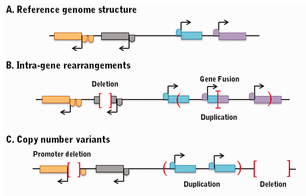
\includegraphics[width=0.5\textwidth,keepaspectratio]{images/rearrangement1.png}}
    \subfloat{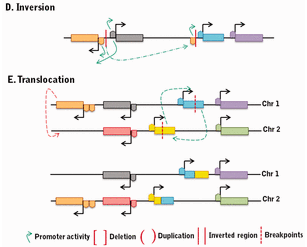
\includegraphics[width=0.4\textwidth,keepaspectratio]{images/rearrangement2.png}}
    \caption[Réarrangement et implication]{\textbf{Réarrangement et conséquences des variants structuraux.} (A) Région génomique sans SV. Les rectangles représentent les gènes et les petits connecteurs à côté représentent le promoteur du gène concerné. (B) Réarrangement intragénique illustrant la délétion et la fusion de gènes à la suite d'une duplication partielle du gène. Les régions codantes modifiées produisent des transcrits aberrants. La délétion ou la duplication peut entraîner une modification du nombre des gènes dans des régions par ailleurs fonctionnellement intactes. (C) Délétion du promoteur, la régulation est modifiée et une duplication/délétion qui modifie le nombre de copies des gènes. (D) Inversions affectant la structure du gène, le gène est inversé, retourné et réarrangé, ce qui éloigne l'un des promoteurs du premier gène (orange). (E) Translocations affectant le contexte génique. Figure extraite et adaptée de \cite{periwal_insights_2015}}
    \label{fig:rearrangement}
\end{figure}

Les recombinaisons peuvent également conduire à la duplication de gènes ou de régions génomiques, un mécanisme clé dans l’évolution des procaryotes en générant une redondance génétique. Cette redondance offre une opportunité évolutive : tandis qu’une copie du gène conserve sa fonction initiale, l’autre peut accumuler des mutations, potentiellement aboutissant à une nouvelle fonction, sans compromettre la survie de l’organisme. En outre, la duplication peut jouer un rôle dans la régulation de l’expression génique. Par exemple, les gènes codant pour les pompes à efflux, impliquées dans l’évacuation des antibiotiques hors de la cellule, sont fréquemment dupliqués, favorisant ainsi une meilleure résistance aux traitements \cite{maddamsetti_duplicated_2024}. Toutefois, les événements de duplication restent moins fréquents que les transferts horizontaux de gènes dans les génomes procaryotes \cite{tria_gene_2021}. Cette rareté s’explique en partie par les mécanismes d’élimination de la redondance, qui optimisent la compacité et l’efficacité des génomes bactériens.

Les mécanismes qui viennent d'être décrits apportent de l'innovation dans les génomes procaryotes, qui doit ensuite être transmise dans la population. Avec le transfert vertical, cette transmission se fait uniquement d'une génération à l'autre, un processus limité par le temps de génération, qui varie selon l'espèce (\textit{E. coli} : 20 min, \textit{Lactobacillus acidophilus} : 80 min, \textit{Mycobacterium tuberculosis} : 800 min). Un temps de génération plus long semble aussi réduire le taux de mutation spontanée de l'ADN \cite{weller_generation-time_2015}. Pour contourner ces contraintes, les procaryotes échangent de l’ADN avec leur environnement (autres bactéries, virus, eucaryotes, ADN libre\dots), par un ensemble de processus regroupé sous le terme de \textbf{transfert horizontal}, qui leur permet d’acquérir de nouvelles fonctions génétiques.

\subsection{Mécanismes d'évolution par transfert horizontal}
\label{sec:evo_hz}

Les transferts horizontaux de gènes (\textit{Horizontal Gene Transfert} en anglais, HGT) constituent un phénomène central dans l'évolution des procaryotes, permettant l'échange de matériel génétique entre organismes sans nécessiter une relation de lignage directe. La proportion de gènes acquis par transfert horizontal varie considérablement selon les espèces et les environnements, mais elle peut représenter une part significative du génome procaryote. On estime que 20 \% des gènes en moyenne ont été acquis par HGT, certaines études montent même jusqu'à 25 \% pour certaines bactéries \cite{ochman_lateral_2000,popa_directed_2011}. Cette proportion élevée témoigne de l'importance des HGT dans l'évolution et l'adaptation des procaryotes.

Les gènes sont transférés via des éléments génétiques mobiles (MGE), incluant les plasmides, les transposons et les phages (virus de bactérie, cf. \autoref{sec:phage}), chacun possédant des capacités uniques pour mobiliser les gènes. Ces vecteurs facilitent le transfert et l'intégration de l'ADN étranger dans le génome hôte. Les séquences répétées, telles que les insertions et les répétitions en tandem, jouent également un rôle, en servant de sites d'intégration pour les MGE. 

Il existe 3 grands mécanismes de HGT : la \textbf{transformation}, la \textbf{conjugaison} et la \textbf{transduction}, chacun facilitant le mouvement de gènes entre cellules de manière distincte.

\subsubsection{Conjugaison : la sexualité des procaryotes}

La conjugaison a été découverte en 1946 par Joshua Lederberg et Edward L. Tatum \cite{lederberg_sex_1953}, qui décrivent ce mécanisme comme la manière sexuée des bactéries d'échanger de l'ADN. En effet, par analogie, la conjugaison demande un contact direct entre une cellule donneuse et une cellule receveuse pour l'échange de matériel génétique\footnote{N.B : Le transfert est unidirectionnel, la cellule donneuse ne peut recevoir de l'ADN et la receveuse ne peut en donner.}. Il existe 2 catégories d'éléments génétiques mobiles conjugatifs : les plasmides et les éléments intégratifs et conjugatifs (ICEs, \textit{Intergrative and Conjugative elements} en anglais). Sur la \autoref{fig:conjugaison} est représenté l'échange d'un plasmide par conjugaison. Les ICEs \cite{johnson_integrative_2015}, contrairement aux plasmides, sont directement intégrés au chromosome, ce qui rend leur réplication dépendante  de celui-ci. Toutefois, cette intégration favorise un transfert vertical plus stable au cours des générations. Les ICEs pour être échangés doivent suivre un schéma circulaire : excision du chromosome, circularisation, réplication, transfert et réintégration dans le chromosome. Lors de l'étape d'excision, il peut arriver que des gènes flanquant l'ICEs soient excisés aussi, apportant une nouvelle forme à l'ICE \cite{gibbons_genomic_2011}.

\begin{figure}[htbp]
    \centering
    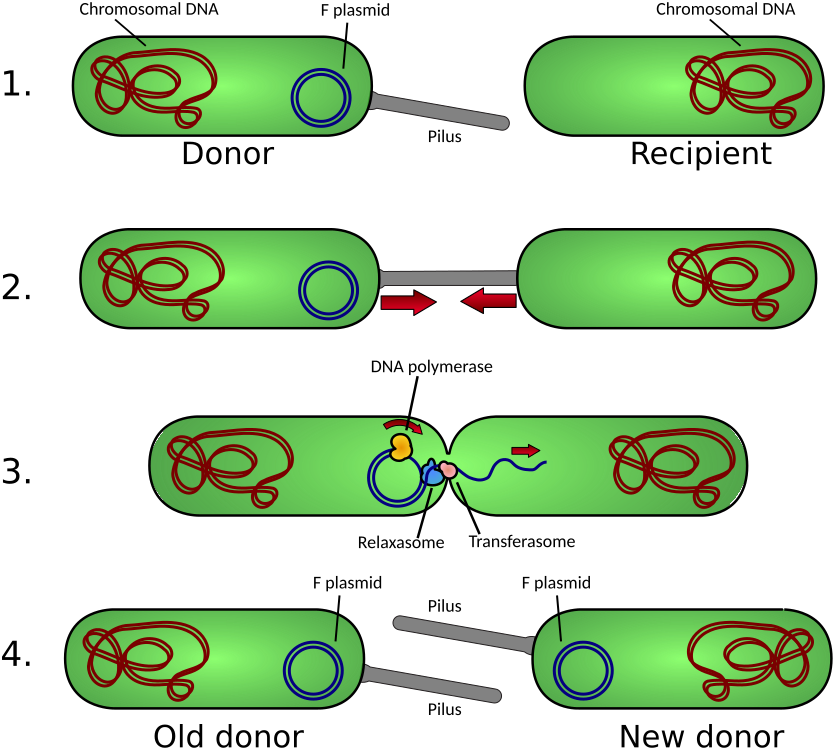
\includegraphics[width=0.7\linewidth]{images/Conjugation.png}
    \caption[Schéma du fonctionnement de la conjugaison]{\textbf{Schéma du fonctionnement de la conjugaison, dans le cas d'un plasmide conjugatif.} (1) Formation d'un pili sexuel par la bactérie donneuse. (2) Contact direct entre les 2 bactéries via le pili. (3) Réplication de l'ADN plasmidique et transfert à la bactérie donneuse. (4) Terminaison de la conjugaison et nouvelle formation d'un pili pour la receveuse devenue donneuse. Image sous licence Creative Commons 3.0 \url{https://commons.wikimedia.org/wiki/File:Conjugation.svg}}
    \label{fig:conjugaison}
\end{figure}

Plasmides et ICEs sont généralement de petite taille, mais ils contiennent des gènes clés d'adaptation à l'environnement. La présence de ces gènes dans les éléments mobiles permet à des colonies de répondre efficacement et rapidement aux nouvelles conditions environnementales, comme la présence de métaux lourds ou d'antibiotiques \cite{botelho_role_2021}. Toutefois, tous les MGEs ne sont pas forcément conjugatifs \cite{valentine_mobilization_1988}, ils vont profiter de la conjugaison codée par un autre élément pour se transférer. Dans ces conditions, la bactérie receveuse ne devient pas conjugative à son tour, même si elle reçoit l'élément mobile. Ces éléments mobilisables sont appelés des IMEs (élément intégratif mobilisable). Il est d'ailleurs à noter que tous les plasmides ne sont pas mobilisables, il y aurait d'ailleurs autant de plasmides conjugatifs que de plasmides non mobilisables \cite{smillie_mobility_2010}.

La conjugaison est un mécanisme majeur de transfert horizontal de matériel génétique, qui a la caractéristique de rapidement répandre les éléments mobiles. Il a toutefois le défaut de limiter le transfert de gènes entre cellules procaryotes et donc de limiter le transfert aux innovations génétiques déjà intégrées par un autre organisme procaryote. De plus, tous les organismes ne sont pas capables de réaliser la conjugaison, ce qui réduit d'autant plus la capacité de transfert au niveau des communautés.

\newpage
\subsubsection{Transformation : recycler l'ADN environnant}

La transformation correspond à l'intégration d'un fragment d'ADN étranger dans le génome de l'organisme. Les bactéries pouvant réaliser la transformation sont dites compétentes. Ce qui  différencie la transformation de la conjugaison, c'est que l'ADN intégré est libre dans l'environnement
\footnote{La découverte de la transformation en 1928 par Fred Griffith \cite{griffith_significance_1928}, précède de nombreuses années celle qui a mis en évidence que l'ADN est le porteur de l'information génétique \cite{avery_studies_1944}. La transformation est donc une preuve anticipée et un socle pour démontrer le rôle de l'ADN.}. De plus, la transformation est la seule forme de HGT, totalement contrôlée par la cellule receveuse \cite{huang_activation_2021}. Assez peu d'espèces sont connues pour être capables de réaliser la transformation de manière naturelle, toutefois un nombre plus important contient  la machinerie nécessaire à sa réalisation \cite{johnston_bacterial_2014}. De plus, au sein d'une espèce, le taux d'individu compétent peut varier, par exemple chez \textit{S. pneumoniae}, 66 \% des individus sont capables de la réaliser \cite{evans_significant_2013}.
Pour terminer, les mécanismes de la transformation, notamment l’incorporation de l’ADN dans la cellule (\autoref{fig:transformation}), sont bien décrits dans la littérature \cite{johnston_bacterial_2014,dubnau_mechanisms_2019}. Toutefois, ils varient d’une espèce procaryote à l’autre, tout comme la proportion d’individus capables de réaliser cette transformation \cite{stewart_biology_1986}. Nous ne reviendrons donc pas sur les mécanismes, mais seulement sur des exemples d'application.

\begin{figure}[htbp]
    \centering
    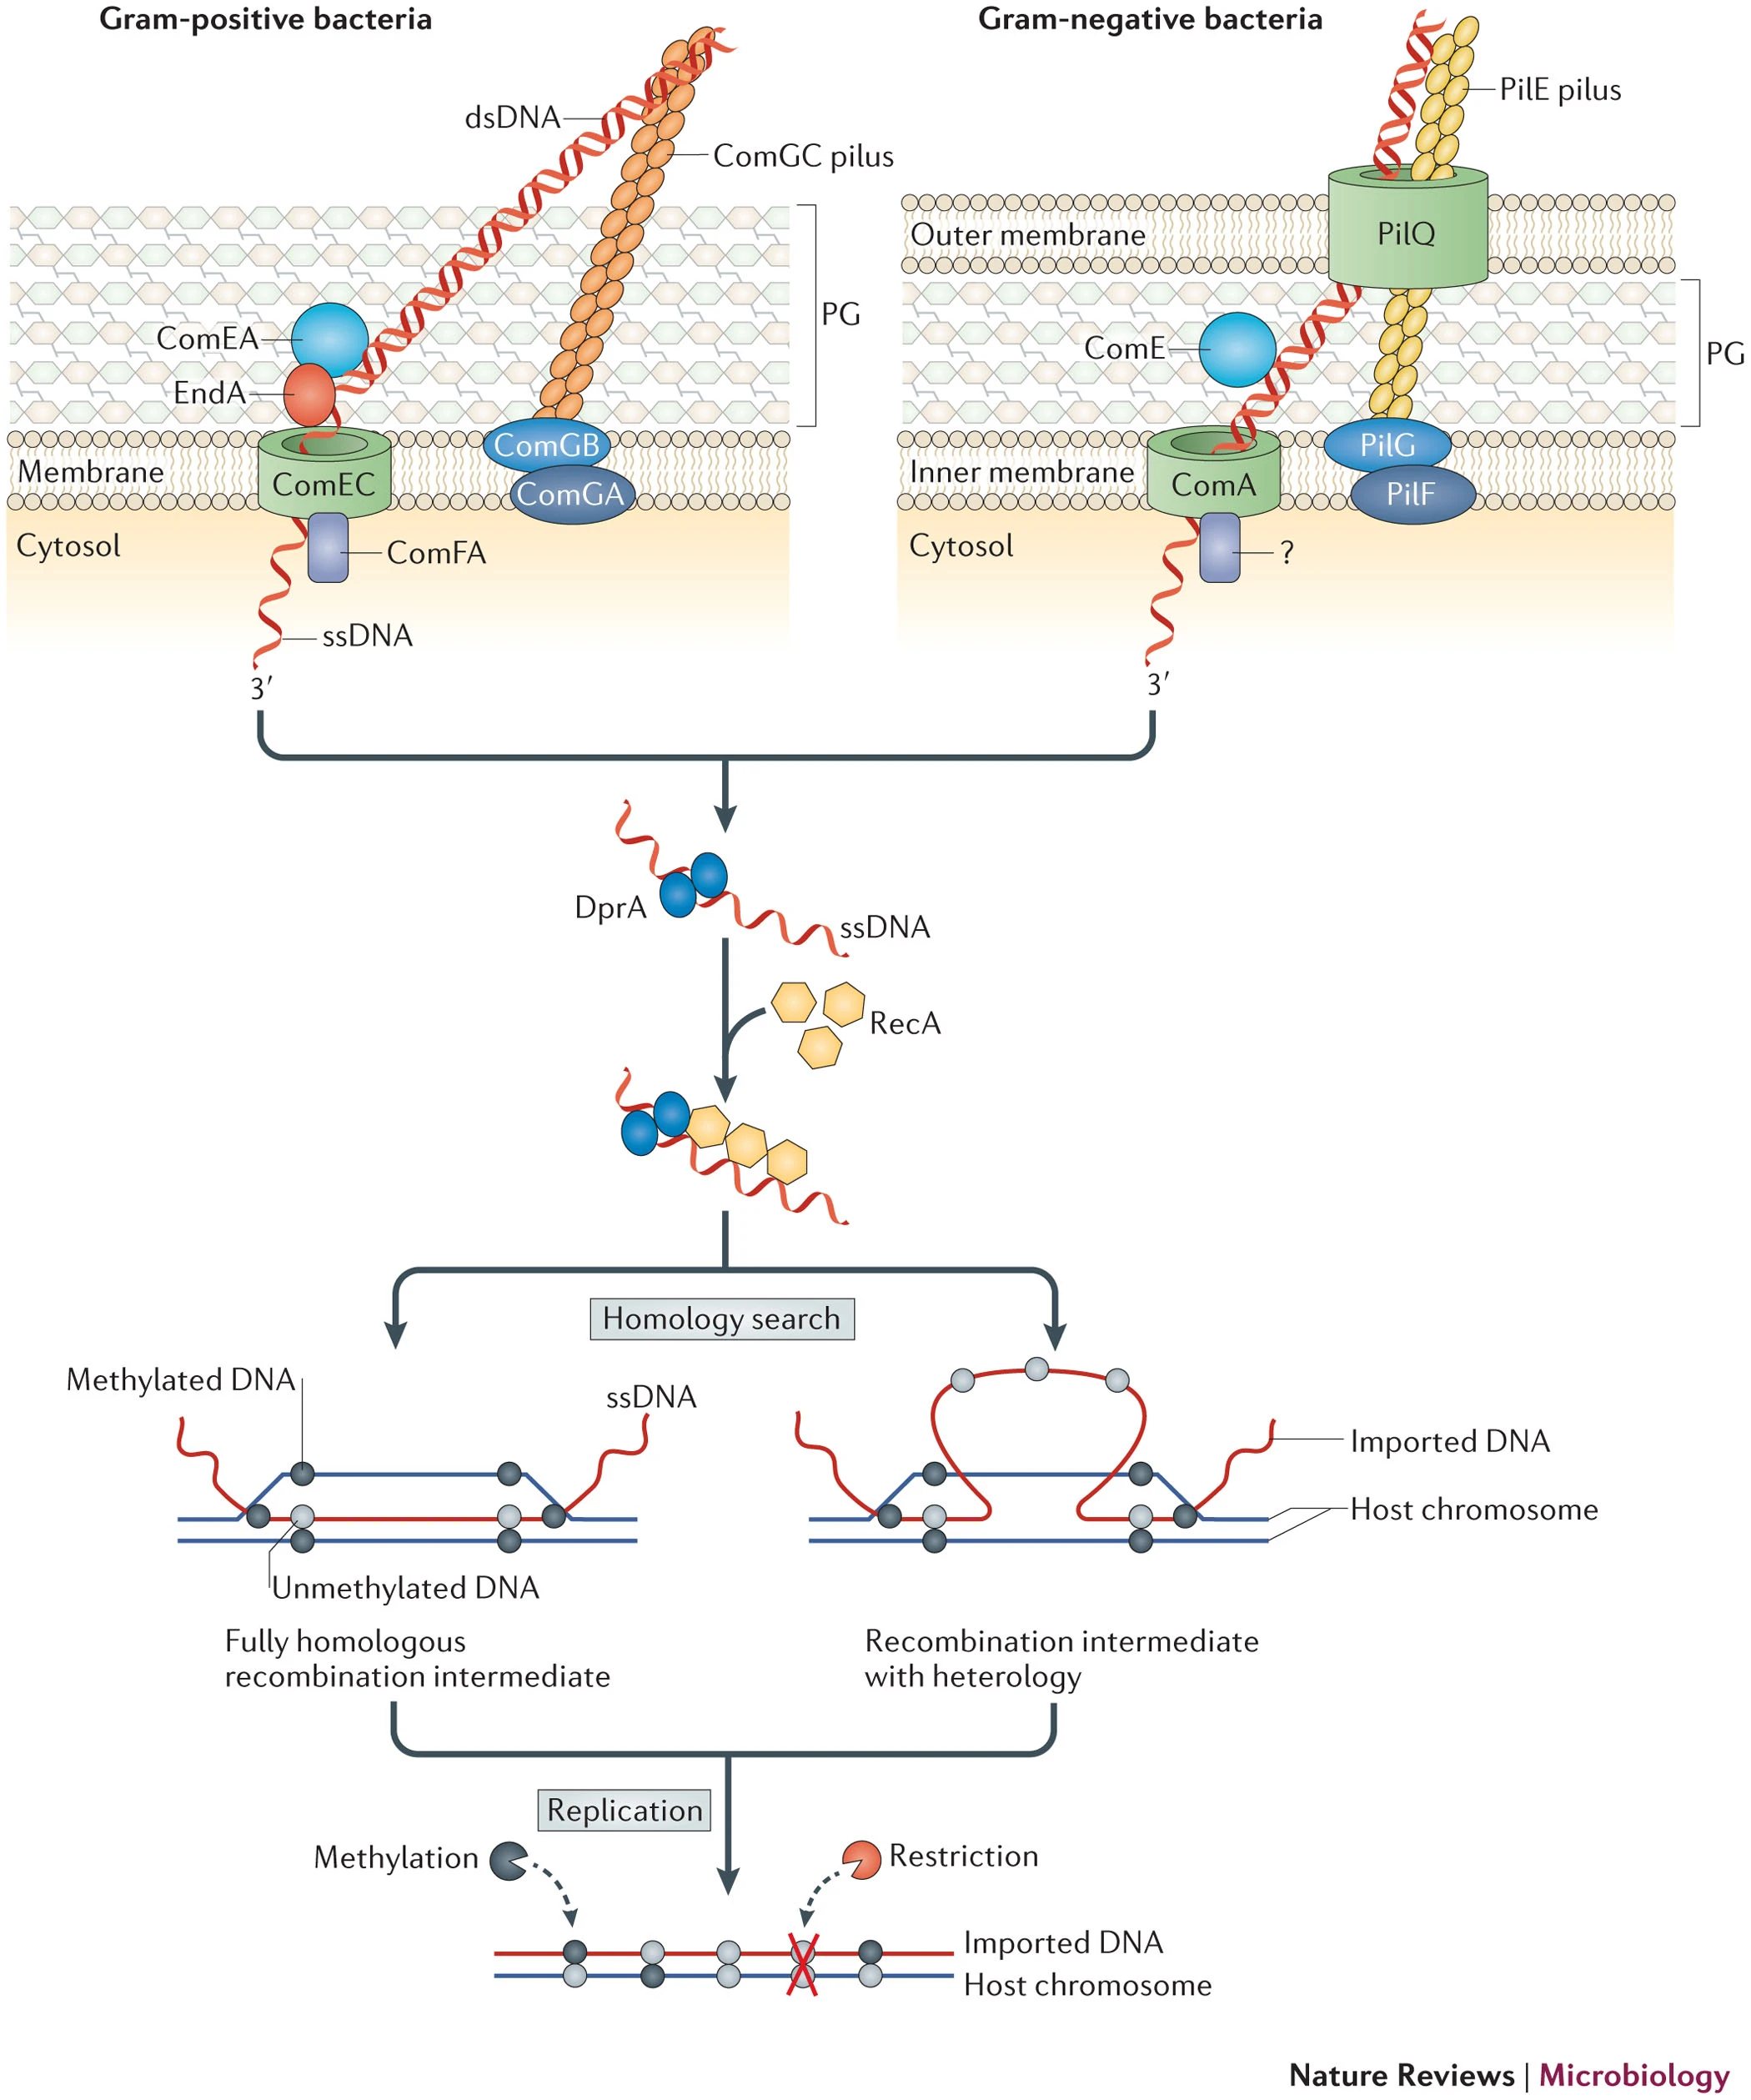
\includegraphics[width=0.625\linewidth]{images/transformation.png}
    \caption[Schéma du mécanisme de transformation]{\textbf{Schéma du mécanisme de transformation.} Extrait de \cite{johnston_bacterial_2014}}
    \label{fig:transformation}
\end{figure}

Les bactéries du genre \textit{Nesseria} et particulièrement \textit{N. gonorrhoeae}\footnote{Ce genre bactérien, vivant dans les muqueuses des mammifères, est non pathogène à l'exception de \textit{N. meningitidis}, impliqué dans la méningite et \textit{N. gonorrhoeae}, responsable de la gonorrhée, une infection sexuellement transmissible.} reconnaissent préférentiellement une séquence d'ADN non palindromique de leur propre ADN \cite{goodman_identification_1988,duffin_dna_2010}. Ce système permet d'intégrer uniquement l'ADN de souches proches, ainsi que des gènes d'adaptation, comme des gènes de résistance aux antibiotiques \cite{centers_for_disease_control_and_prevention_cdc_update_2007}. Ainsi, les gènes d'adaptation d'intérêt sont préférentiellement distribués dans l'espèce.

\textit{Streptococcus pneumoniae}\footnote{Bactérie connue pour son rôle d'agent pathogène dans les pneumonies et responsable de co-infection pendant la grippe espagnole} utilise la transformation comme mécanisme de réparation de l'ADN, car cette espèce ne possède pas de système de réparation SOS \cite{gasc_lack_1980}. Les souches de \textit{S. pneumoniae} s'engagent alors dans une "guerre fratricide" pour récupérer l'ADN des autres souches de leur espèce \cite{claverys_cannibalism_2007}.

Pour terminer, chez \textit{Bacillus subtilis}\footnote{Bactérie du sol, mais qu'on retrouve dans de nombreux habitat dû à ses capacités d'adaptation. Elle est utilisée comme modèle d'étude des bactéries Gram+.}, la transformation entre individus de la même espèce, mais de souche éloignée, est privilégiée \cite{lyons_combinatorial_2016}. Les bactéries vont sécréter dans l'environnement des antibiotiques, auxquels elles sont résistantes, pour tuer les autres individus de l'espèce. L'ADN récupéré est donc différent de celui de la bactérie et donc potentiellement source de nouvelles fonctions.

Ces exemples montrent aussi une opposition dans la philosophie des mécanismes de conjugaison et de transformation. La transformation demande que l'ADN soit libre dans l'environnement et donc que les bactéries environnantes soient détruites, alors que la conjugaison laisse les 2 cellules en vie. 

\subsubsection{Transduction : les virus mis à profit}

La transduction est un mécanisme reposant sur l'intervention d'un virus pour transporter et transférer le matériel génétique d'une cellule procaryote à l'autre (\autoref{fig:transduction}). Les virus de bactéries, surnommés (bacterio)phages, vont infecter la cellule donneuse pour répliquer leur ADN. Lors de la réplication, de l'ADN de la cellule donneuse peut se trouver intégré à celui du phage. Lorsqu'il infectera une cellule receveuse, la portion d'ADN de la donneuse pourra reprendre une forme plasmidique (si c'est un plasmide qui a été transféré) ou être intégrée au génome de la cellule par recombinaison homologue. La transduction est aujourd'hui largement utilisée en génétique et microbiologie pour transférer de l'ADN et modifier les génomes \cite{wang_phage-based_2024}. 

\begin{figure}[htbp]
    \centering
    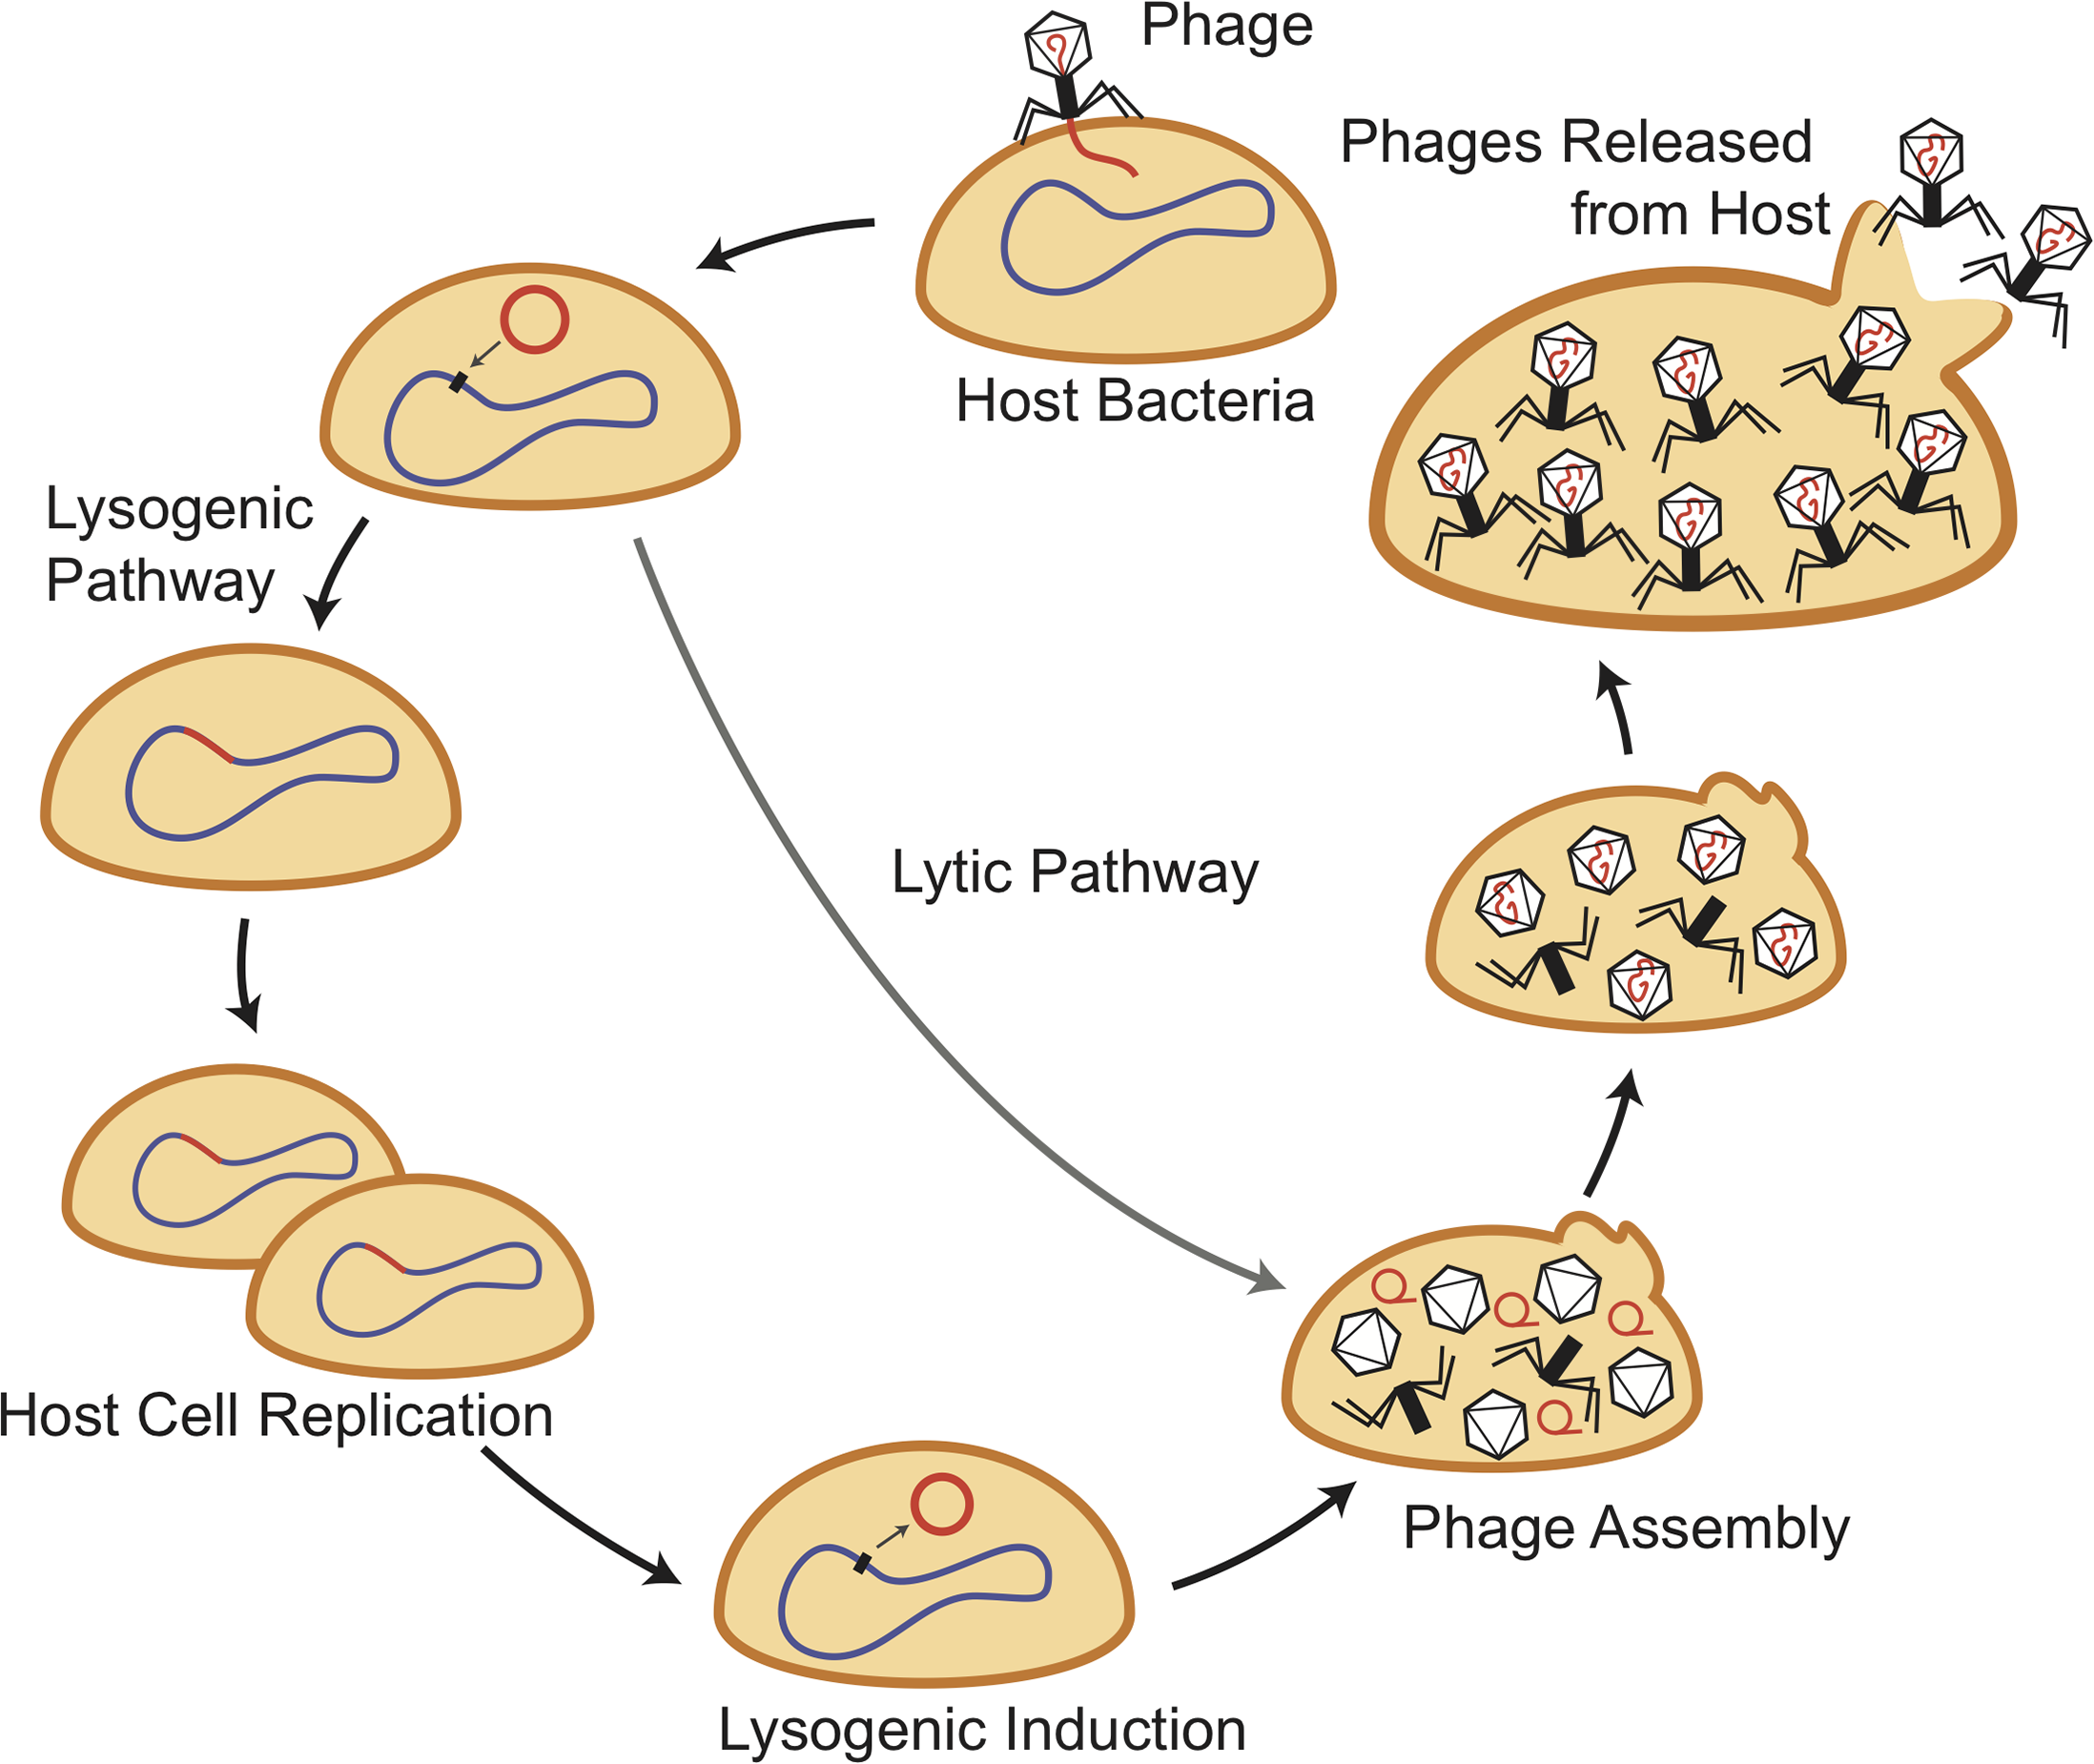
\includegraphics[width=0.65\linewidth]{images/transduction.png}
    \caption[Schéma synthétique de la transduction]{\textbf{Schéma représentant les étapes de transduction.} Extrait de \cite{chiang_genetic_2019}}
    \label{fig:transduction}
\end{figure}

La première forme de transduction identifiée décrivait le transfert de n'importe quel gène de la donneuse à la receveuse par le phage. Cette forme a donc été nommée transduction généralisée \cite{zinder_genetic_1952}. Une seconde forme dite spécifique a été découverte en étudiant le phage $\lambda$ infectant les \textit{E. coli} \cite{morse_transduction_1956}. Le transfert se limite à un ensemble de gènes définis. Enfin, une dernière forme, la transduction latérale, a récemment été découverte \cite{chen_genome_2018}. Là où les formes générale et spécifique peuvent être vues comme une erreur et un événement lié au hasard, la transduction latérale fait partie du cycle de vie du phage, menant à un taux de transfert beaucoup plus important. 

\newpage
\section{Du génome aux processus cellulaires}

\subsection{Gènes : Régulations et fonctions}
\label{sec:fn_reg}

Les réactions qui se produisent dans les cellules procaryotes sont souvent complexes et impliquent une multitude de réactifs et de produits. Toutes ces réactions nécessitent la présence de protéines spécifiques pour être réalisées. Ces protéines sont produites et dégradées par la cellule en fonction des conditions rencontrées. C'est pourquoi l'information est stockée dans une structure durable et transmissible, le gène. Chaque gène sera transcrit en une molécule d'ARN messager (ARNm) par l'ARN polymérase, qui sera traduite en protéine par le ribosome (impliquant l'ARNr et l'ARNt). 


Dans une cellule, les protéines ont un temps de "vie" allant de quelques minutes à quelques heures. Il est donc nécessaire de produire les protéines régulièrement, toutefois cette production a un coût pour la cellule. C'est pourquoi il existe des mécanismes de régulation de l'expression des gènes et donc de la production des protéines. Dans la \autoref{sec:gene}, nous avons vu qu'il existait notamment des petits ARN régulateurs de l'expression. Dans l'ADN non codant, on retrouve également une séquence promotrice (ou promoteur) près d'un gène qui permet la fixation de l'ARN polymérase. La fixation et l'activation de l'ARN polymérase au niveau du promoteur sont régulées par des facteurs de transcription qui se lient spécifiquement à des séquences régulatrices en amont du promoteur, les \textit{enhancer} et \textit{silencer}.


Les protéines peuvent agir en collaboration, soit dans des réactions successives (cas des systèmes biologiques, cf. \autoref{sec:sys_bio}), soit en formant des complexes protéiques interagissant pour métaboliser un produit. Les gènes codant pour des protéines impliquées dans les mêmes processus cellulaires sont situés dans le même contexte génomique (cf. \autoref{sec:gene}). Ils vont alors être régulés par les mêmes éléments de régulation. L'opéron, une structure spécifique des procaryotes découverte par François Jacob et Jacques Monod en 1960\footnote{Découverte qui leur a valu le prix Nobel de médecine en 1965}\cite{jacob_genetic_1961}, permet de produire un seul ARNm pour un ensemble de gènes codant pour des protéines impliquées dans le même processus cellulaire. Dans l'opéron, se trouve une nouvelle séquence de régulation, l'opérateur, où va se lier une molécule régulatrice qui va activer ou inhiber la transcription (\autoref{fig:lac_operon}). L'ensemble de l'opéron permet de synchroniser la régulation et l'expression de gènes qui collaborent dans le même processus cellulaire.


\begin{figure}[htbp]
    \centering
    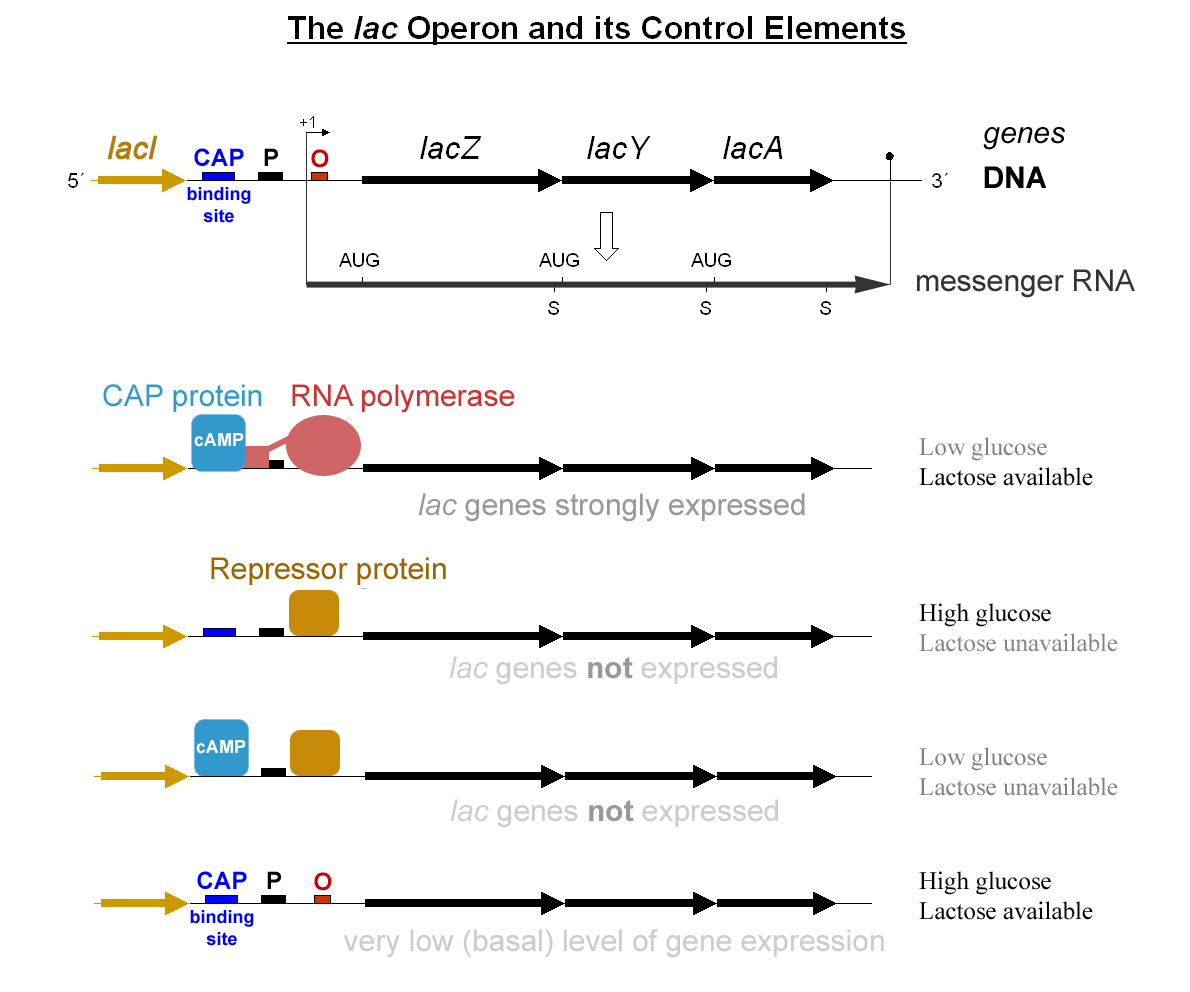
\includegraphics[width=\linewidth]{images/Lac_operon-2010-21-01.png}
    \caption[Exemple de l'opéron lactose]{\textbf{Schéma du fonctionnement de l'opéron lactose.} Sur la partie haute est représenté la structure génétique de l'opéron. Les 4 lignes suivantes représentent chacune une configuration de réponse à des conditions de présence, absence de glucose et de lactose. si le taux de glucose est faible, une protéine activatrice (CAP) va se fixer en amont du promoteur pour aider à la fixation de l'ARN polymérase, et si du lactose est disponible, les gènes seront alors fortement exprimés. Si le lactose n'est pas disponible, une protéine de répression va se fixer à l'opérateur et elle empêchera l'ARN polymérase de se fixer même si le taux de glucose est faible. 
    Auteur : G3pro. Sous licence Creative Commons 2.0. Disponible à l’adresse : \url{https://commons.wikimedia.org/wiki/File:Lac_operon-2010-21-01.png.}
    }
    \label{fig:lac_operon}
\end{figure}

Pour terminer, l'expression des gènes peut aussi être régulée par le niveau de repliement et de condensation de l'ADN. L'ADN est condensé notamment grâce à des protéines spécialisées et à la méthylation de l’ADN. L'ADN replié ne pourra pas être accessible pour la transcription des gènes et donc ils seront inactifs. Les mécanismes liés à la méthylation de l'ADN sont l'affaire de l’épigénétique. Des études récentes ont mis en lumière le rôle de la méthylation dans la régulation de la virulence bactérienne et dans la capacité des procaryotes à coloniser leurs hôtes \cite{oliveira_bacterial_2021}, soulignant ainsi l'importance de ces mécanismes dans la survie et l’adaptation des bactéries.

\newpage
\subsection{Îlots génomiques et points chauds d'insertion}
\label{sec:ilot}
Les îlots génomiques (GI, pour \textit{Genomic Island en anglais}) sont des régions spécifiques du génome qui jouent un rôle clé dans l'évolution, l'adaptation et l'acquisition de fonctions spécifiques. Les GIs sont retrouvés chez quasiment tous les organismes procaryotes. Ils sont généralement acquis par transfert horizontal (cf. \autoref{sec:evo_hz}) et transportent des gènes accessoires. Ils vont conférer à l'organisme de nouvelles fonctions qui impacteront de façon positive sa \textit{fitness}. Le premier îlot génomique décrit était lié à la capacité de la bactérie \textit{E. coli} de provoquer des maladies et a donc été nommé îlot de pathogénicité \cite{hacker_deletions_1990}.  Depuis, d'autres classes d'îlots ont été découvertes : métabolique, résistance, symbiotique\dots (\autoref{fig:GI}).

Les îlots génomiques sont des régions assez larges, entre 5 et 200 kb (mais certaines sont beaucoup plus grandes) et présentent des caractéristiques spécifiques. (\textit{i}) Les GIs ont un taux de GC qui diffère par rapport au reste du génome, résultant en un biais d'usage des codons\footnote{Un biais d'usage des codons, désigne la fréquence d’utilisation préférentielle de certains codons parmi les codons synonymes pour coder un même acide aminé.} (\autoref{fig:GI}). (\textit{ii}) dans les régions flanquantes des GIs, on retrouve des gènes de mobilité : transposases et intégrases, mais aussi d'IS qui peuvent se dégrader rapidement après l'intégration de l'îlot. (\textit{iii}) Dans les gènes flanquants, on retrouve des gènes codant l'ARNt dont l'origine serait à relier à la prévalence des gènes de phages et des ICEs qui utilisent les ARNt comme site d'intégration dans les génomes \cite{dobrindt_genomic_2004}. (\textit{iv}) Les protéines contenues dans les GIs ont souvent des fonctions inconnues. (\textit{v}) Dans la partie flanquante, on trouve des séquences répétées directes\footnote{Séquences identiques présentes en plusieurs copies dans la même molécule d'ADN et ayant la même orientation.}.

\begin{figure}[htbp]
    \centering
    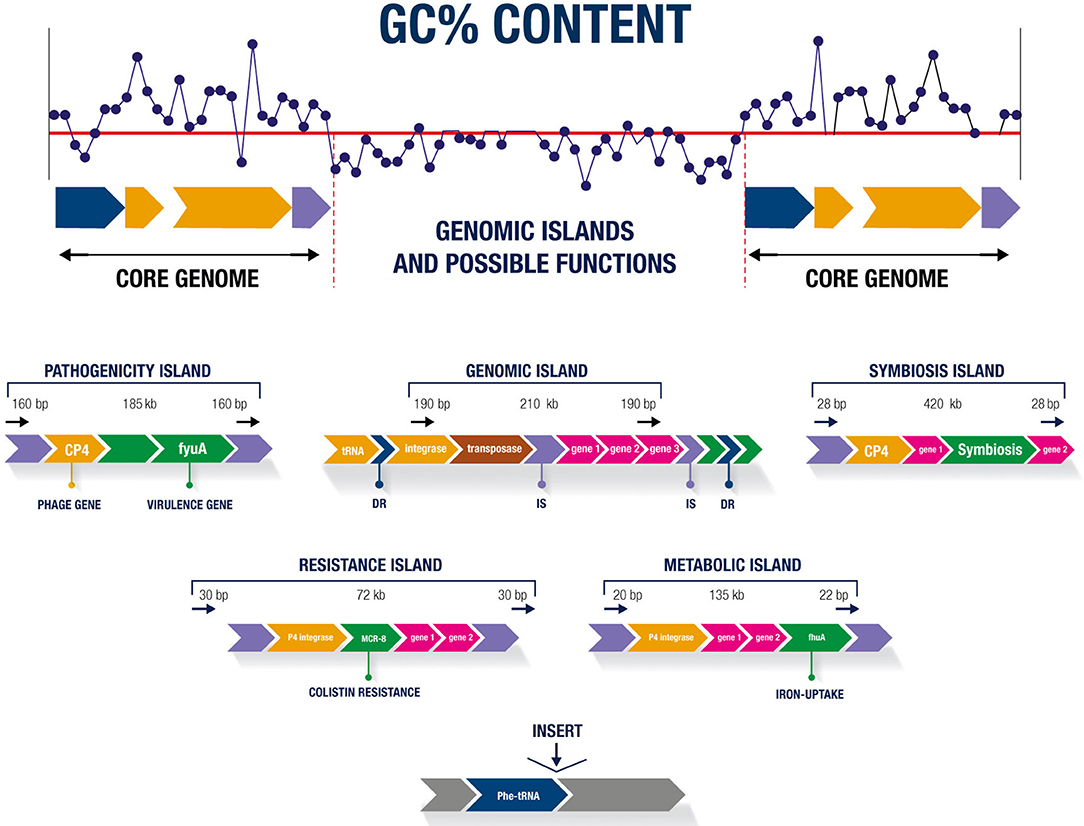
\includegraphics[width=0.8\linewidth]{images/ilot_genomique.jpg}
    \caption[Îlots génomiques et leur caractéristique]{\textbf{Îlots génomiques et leur caractéristique.} Extrait de  \cite{da_silva_filho_comparative_2018}}
    \label{fig:GI}
\end{figure}

\newpage
Ces GIs sont complexes à étudier, car ils concentrent les variations, même entre génomes proches. L'histoire évolutive est souvent difficile à reconstituer, tant des éléments ont été intégrés et éliminés au cours du temps (\autoref{fig:cycle_IG}). En plus de s'échanger avec d'autres organismes \cite{buchrieser_high-pathogenicity_1998}, les GIs peuvent se déplacer au sein du génome \cite{karaolis_bacteriophage_1999}.

\begin{figure}[htbp]
    \centering
    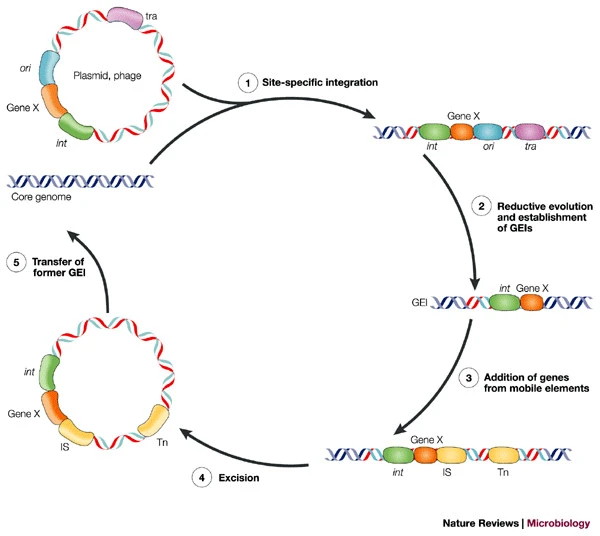
\includegraphics[width=0.65\linewidth]{images/cycle_GI.png}
    \caption[Cycle de vie d'un îlot génomique]{Cycle de vie d'un îlot génomique. Extrait de \cite{dobrindt_genomic_2004}}
    \label{fig:cycle_IG}
\end{figure}

Les GIs ne s'insèrent pas n'importe où dans les génomes. On les retrouve fréquemment dans des zones où de nombreux éléments se sont insérés au cours de l'évolution d'un taxon. Ces régions sont appelées : point chaud d'insertion (\textit{hotspot} en anglais).
À l'intérieur des \textit{hotspots}, on retrouve une grande variabilité du contenu génique entre les génomes. Les \textit{hotspots} sont également caractérisés par des bordures composées de gènes communs à l'ensemble des génomes. 

Ils présentent également une recombinaison homologue accrue dans les gènes flanquant les \textit{hotspots}, avec 50 \% d’événements de recombinaison et 30 \% d’incongruence phylogénétique\footnote{L'incongruence phylogénétique désigne une discordance entre l’arbre phylogénétique d’un gène spécifique et l’arbre phylogénétique global construit à partir d'un grand nombre de gènes conservés.} par rapport à l'arbre des espèces. Ces \textit{hotspots} contiennent 50 \% des gènes acquis par HGT \cite{oliveira_chromosomal_2017}. Ils sont enrichis en gènes liés à la motilité, à la défense, à la transcription, à la réplication et à la réparation de l’ADN \cite{flores_ramos_genomic_2021}.

Le contenu génique du \textit{hotspot} provient d'une accumulation progressive de gènes, comme le suggère le faible pourcentage (8 \%) de \textit{hotspots} composés uniquement de gènes spécifiques à une souche \cite{oliveira_chromosomal_2017}. Cette accumulation peut se faire par bloc de gènes. Ces blocs, conservés dans le \textit{hotspot}, sont appelés modules \cite{lescat_module_2009}. Cette modularité pourrait expliquer l'organisation complexe des îlots génomiques \cite{touchon_organised_2009}.
Les \textit{hotspots}, sont donc communs à un groupe d'organismes, et définis au niveau d'un taxon. Il est donc nécessaire de mener des études de comparaison des génomes pour les identifier.